\documentclass{article}
\usepackage{amsmath,amssymb,amsthm}
\usepackage{graphicx}

\newtheorem{thm}{Theorem}[section]
\newtheorem{lem}[thm]{Lemma}
\newtheorem{definition}[thm]{Definition}
\newtheorem{example}[thm]{Example}
\newtheorem*{remarkstar}{Remark}

% These metadata commands are author annotations, not formal proof evidence.
\providecommand{\uses}[1]{}
\providecommand{\proves}[1]{}
\providecommand{\lean}[1]{}
\providecommand{\leanok}{}

\title{A small QEC source-graph example}
\author{Demonstration fixture}
\date{}

\begin{document}
\maketitle

% 中文说明：本示例测试源文件位置；字符偏移与 UTF-8 字节偏移并不相同。
% \input{this-comment-must-not-be-read}
% \begin{lem}\label{lem:comment-ghost}This is not a lemma.\end{lem}

\section{Binary CSS conventions}
\label{sec:foundations}

% 中文注释先于真实定义，用来检查 source slice 是否使用字符位置。
\begin{definition}[Binary field]
\label{def:gf2}
The field $\mathbb{F}_2$ has elements $0$ and $1$, with addition and
multiplication modulo two. In particular, $1+1=0$.
\end{definition}

\begin{definition}[Binary CSS presentation]
\label{def:css}
\uses{def:gf2}
Let $H_X\in\mathbb{F}_2^{m_X\times n}$ and
$H_Z\in\mathbb{F}_2^{m_Z\times n}$. Rows of $H_X$ specify X-type
stabilizers, and rows of $H_Z$ specify Z-type stabilizers. The binary
commutation condition is
\begin{equation}
\label{eq:css-commutation}
H_X H_Z^{T}=0.
\end{equation}
The columns are labelled data qubits. The field is the one in
Definition~\ref{def:gf2}; the selected generator rows are part of this
presentation.
\end{definition}

\begin{lem}[Pairwise commutation]
\label{lem:css-commutation}
\uses{def:css,def:gf2}
\lean{QEC.Examples.binary_css_commutation}
\leanok
For the convention in Definition~\ref{def:css}, all X-type generators
commute with all Z-type generators if and only if
Equation~\eqref{eq:css-commutation} holds.
\end{lem}

\begin{proof}
\label{proof:css-commutation}
\uses{def:css}
For binary row vectors $x,z$, the Pauli relation gives
\begin{equation*}
X(x)Z(z)=(-1)^{x\cdot z}Z(z)X(x).
\end{equation*}
Thus the pair commutes exactly when its dot product is zero in
$\mathbb{F}_2$. Applying this statement to every pair of generator rows
gives Equation~\eqref{eq:css-commutation}.
\end{proof}

\begin{remarkstar}[Scope of the annotations]
\label{rem:source-only}
The metadata above deliberately includes an author-supplied Lean name
and a completion marker. This fixture does not contain a Lean project,
and neither declaration existence nor proof validity has been checked.
An importer should retain these annotations as source claims.
\end{remarkstar}

\section{An ordinary hypergraph product}
\label{sec:hgp}

The construction below follows the ordinary hypergraph-product setting
of Tillich and Zemor~\cite{TillichZemor2009}. The small parameters later
in this section are an illustrative source claim, not a quoted table
from that paper.

\begin{thm}[Commutation of the block construction]
\label{thm:hgp-css}
\uses{def:css}
Let $H_1\in\mathbb{F}_2^{m_1\times n_1}$ and
$H_2\in\mathbb{F}_2^{m_2\times n_2}$. Define
\begin{align}
\label{eq:hgp-checks}
H_X&=[H_1\otimes I_{n_2}\mid I_{m_1}\otimes H_2^T],\\
H_Z&=[I_{n_1}\otimes H_2\mid H_1^T\otimes I_{m_2}].
\end{align}
Then $H_XH_Z^T=0$ over $\mathbb{F}_2$.
\end{thm}

\begin{proof}
\label{proof:hgp-css}
\uses{def:gf2,lem:css-commutation}
Multiplying the two blocks gives
\begin{equation}
\label{eq:hgp-commutation}
H_XH_Z^T=H_1\otimes H_2^T+H_1\otimes H_2^T=0.
\end{equation}
The last equality uses the field in Definition~\ref{def:gf2}.
Lemma~\ref{lem:css-commutation} identifies this binary identity with
pairwise commutation of the CSS generators.
\end{proof}

\begin{thm}[Length of the repetition-seed instance]
\label{thm:hgp-length}
Use the construction of Theorem~\ref{thm:hgp-css} with
\begin{equation}
\label{eq:repetition-seed}
H_1=H_2=
\begin{pmatrix}
1&1&0\\
0&1&1
\end{pmatrix}.
\end{equation}
The resulting presentation has thirteen data qubits.
\end{thm}

For background and motivation, compare Theorem~\ref{thm:hgp-css}.
This reference records a discussion link and is not a declaration
that the following table depends on a proof of that theorem.

\begin{table}[ht]
\centering
\caption{Intended finite-instance values in this source fixture.
The importer does not verify these parameters.}
\label{tab:rep3}
\begin{tabular}{lccc}
Construction & $n$ & $k$ & $d$\\
Ordinary HGP of two repetition seeds & 13 & 1 & 3
\end{tabular}
\end{table}

\begin{figure}[ht]
\centering
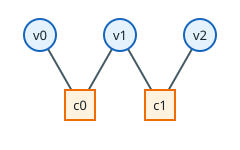
\includegraphics[width=0.6\linewidth]{figures/tanner-placeholder.svg}
\caption{The two-check graph of one length-three repetition seed.
This is not the full thirteen-qubit HGP graph.}
\label{fig:repetition-seed}
\end{figure}

% The proof is intentionally separated from its theorem by prose and floats.
\begin{proof}[Proof of Theorem~\ref{thm:hgp-length}]
\label{proof:hgp-length}
\proves{thm:hgp-length}
\uses{thm:hgp-css}
Each seed in Equation~\eqref{eq:repetition-seed} has $n_i=3$ columns
and $m_i=2$ rows. The first block in
Equation~\eqref{eq:hgp-checks} has $n_1n_2=9$ columns, and the second
has $m_1m_2=4$ columns. Hence $n=9+4=13$.
\end{proof}

\begin{example}[An explicit data claim]
\label{ex:rep3-parameters}
With column order $(i,j)\mapsto 3i+j$ for the first nine qubits and
$(a,b)\mapsto 9+2a+b$ for the remaining four qubits, the intended
instance is $[[13,1,3]]$. The rank and distance values can be checked
by binary linear algebra and exhaustive enumeration.
Table~\ref{tab:rep3} states those values, but this document does not
attach a computation report or a Lean certificate for them.
\end{example}


\section*{Literal examples}
\label{sec:literal-examples}
The following literal source is part of a verbatim example. Its labels and
references must not become mathematical objects or graph references.

\begin{verbatim}
\begin{lemma}
  \label{lem:verbatim-ghost}
  This text is not a mathematical lemma in the document.
\end{lemma}
\ref{thm:verbatim-ghost}
\input{this-verbatim-must-not-be-read}
\end{verbatim}

\bibliographystyle{plain}
\bibliography{references}
\end{document}
